\documentclass{article}

\usepackage{graphicx}
\usepackage{tikz}
\usepackage{tikzsymbols}
\usetikzlibrary{calc,patterns,shapes.geometric}
\pagestyle{empty}
\usepackage[margin=0pt]{geometry}
\geometry{papersize={14in,12in}}

\def\centerarc[#1](#2)(#3:#4:#5){\draw[#1] ($(#2)+({#5*cos(#3)},{#5*sin(#3)})$) arc (#3:#4:#5);}

\begin{document}
	\begin{figure}
		\centering
		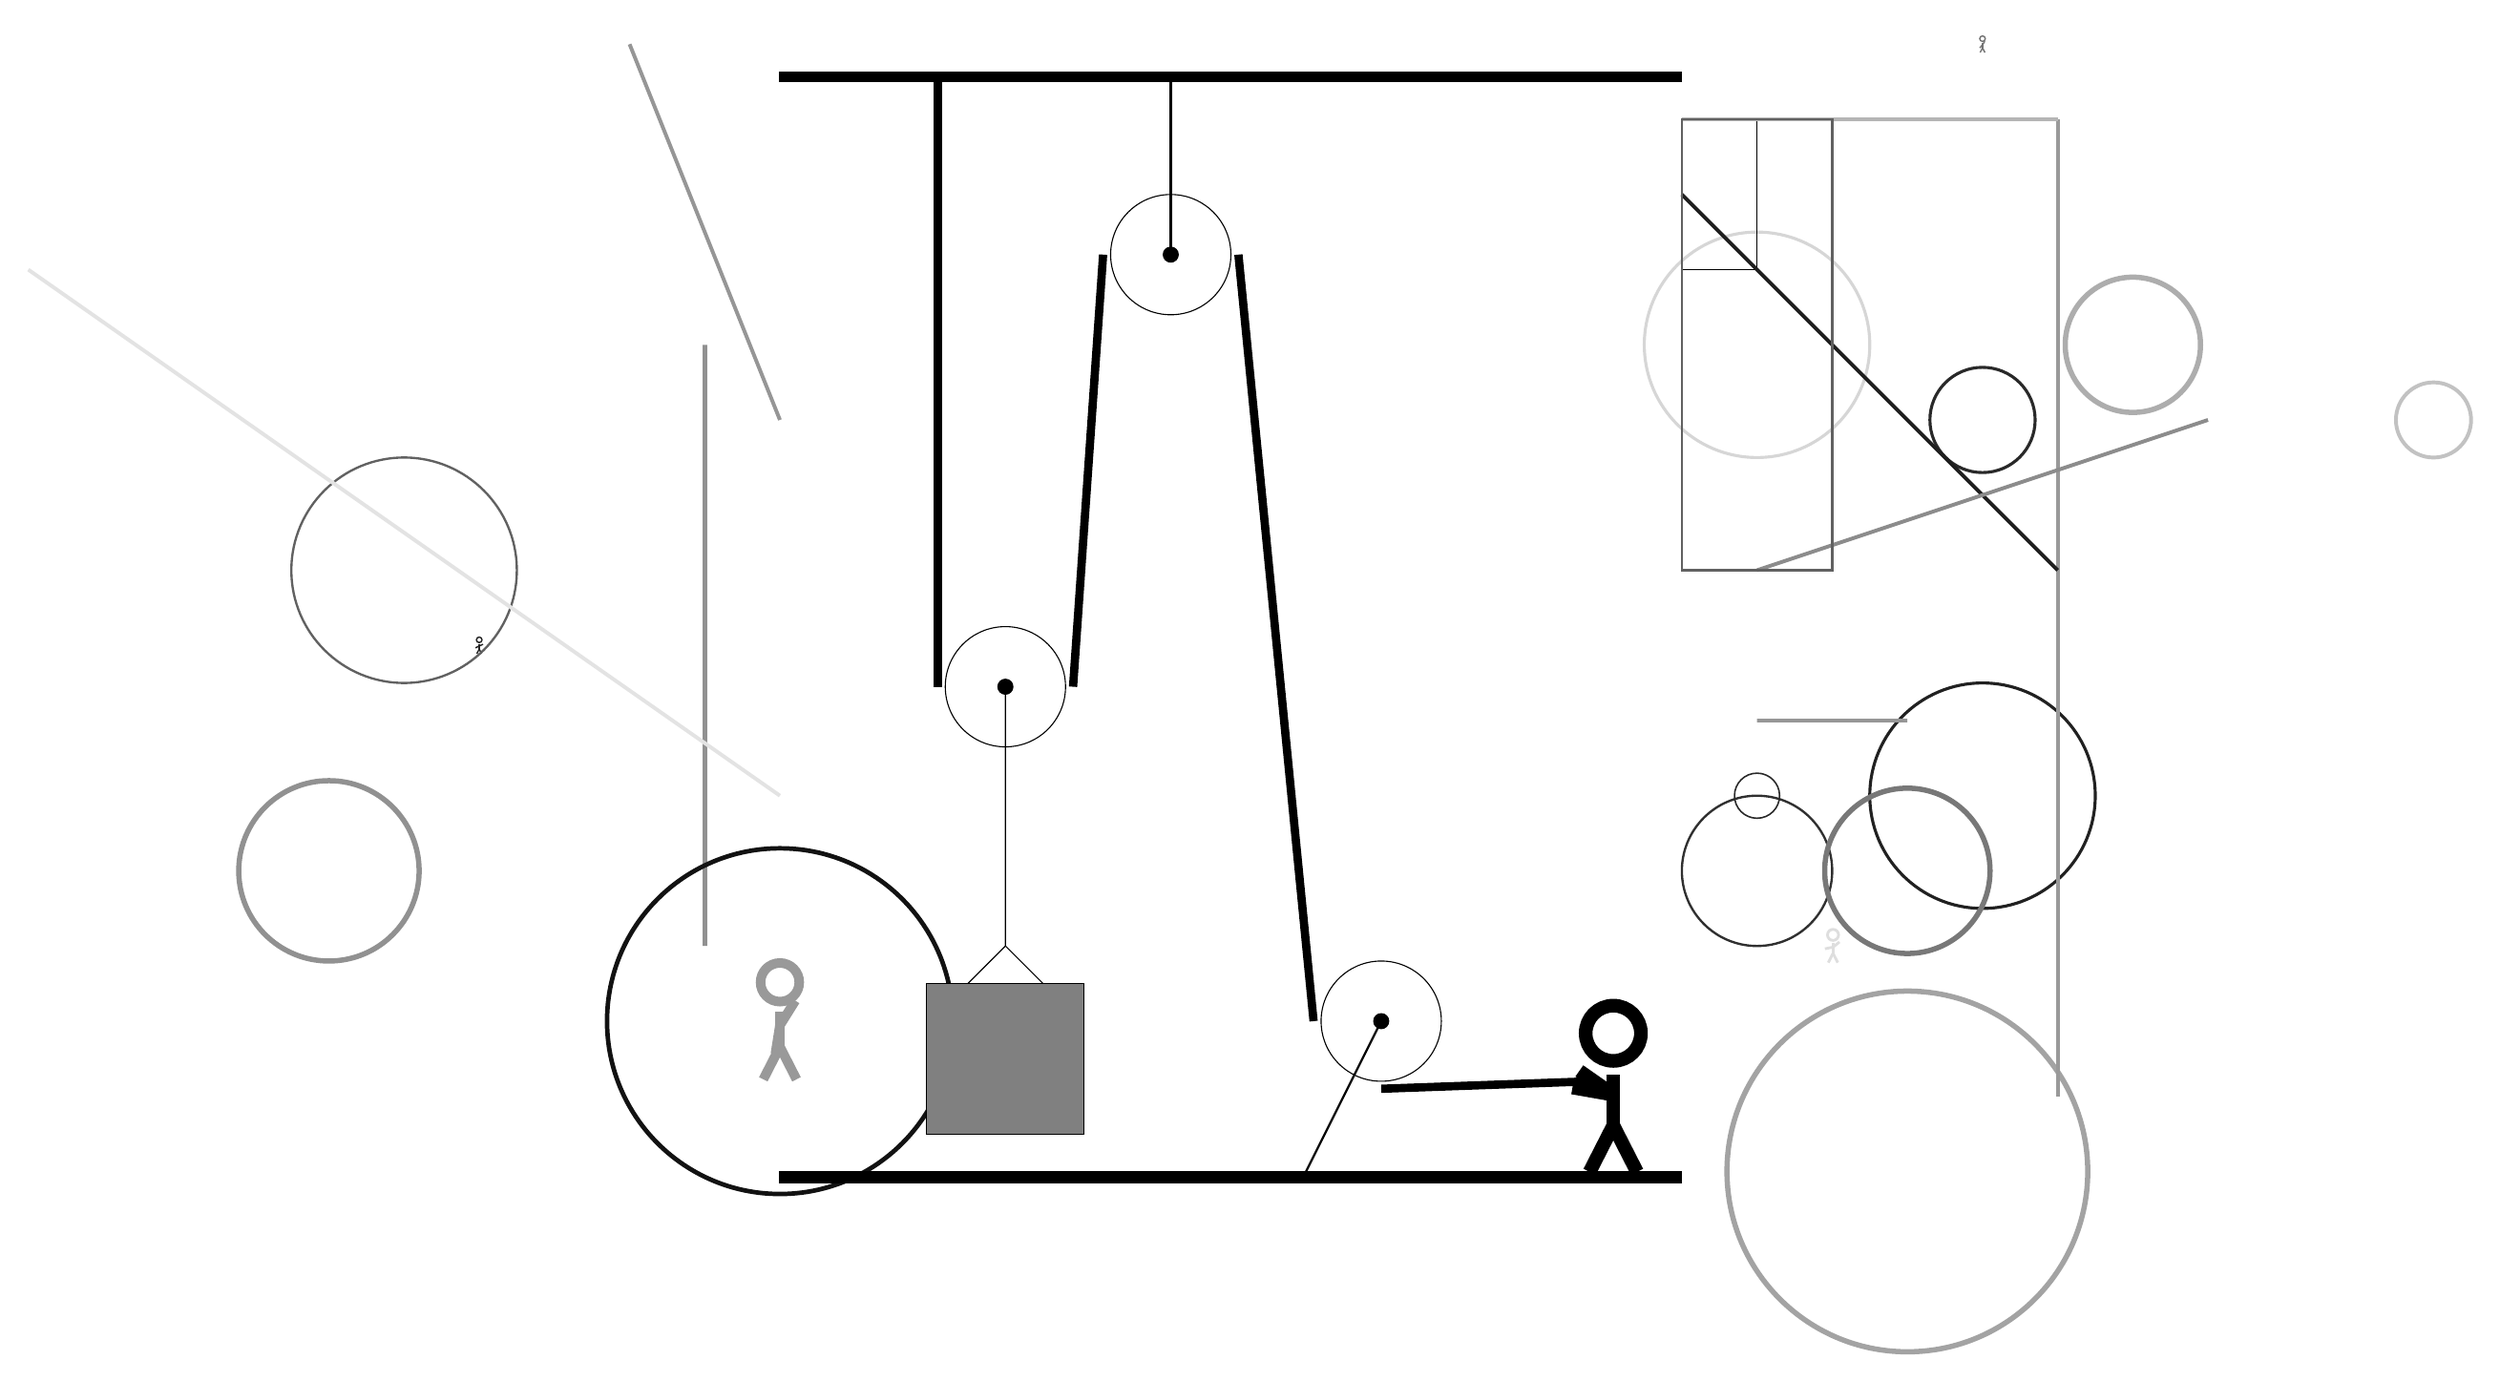
\begin{tikzpicture}
			%%%%% START %%%%%
			
			\draw[fill=black] (-2, 11.5) rectangle (10, 11.625);
			
			\draw (3.2, 9.2) circle (0.8);
			\draw[fill=black] (3.2, 9.2) circle (0.1);
			\draw[thick] (3.2, 9.2) -- (3.2, 11.5);
			
			\draw (6, -1) circle (0.8);
			\draw[fill=black] (6, -1) circle (0.1);
			\draw[thick] (6, -1) -- (5, -3);
			
			\draw [line width=0.7mm, color=black!43](-8, 1) circle (1.2);
			
			\draw [line width=0.4mm, color=black!84](14, 7) circle (0.7);
			\node[line width=0.5mm, color=black!13] at (12, 0) {\Strichmaxerl[2][11][39]};
			\draw [line width=0.4mm, color=black!16](11, 8) circle (1.5);
			\draw [line width=0.3mm, color=black!81](11, 1) circle (1.0);
			
			\node[line width=0.2mm, color=black!86] at (-6, 4) {\Strichmaxerl[1][27][24]};
			
			\draw [line width=0.3mm, color=black!62](-7, 5) circle (1.5);
			
			\draw [line width=0.7mm, color=black!36](13, -3) circle (2.4);
			\draw [line width=0.4mm, color=black!87](14, 2) circle (1.5);
			\draw [line width=0.2mm, color=black!84](11, 2) circle (0.3);
			\draw[line width=0.2mm, color=black!100] (10, 9) rectangle (11, 11);
			\draw [line width=0.7mm, color=black!32](16, 8) circle (0.9);
			\draw[line width=0.5mm, color=black!40](15, 11) -- (15, -2);
			
			\draw[line width=0.5mm, color=black!41] (11, 3) rectangle (13, 3);
			\draw[line width=0.6mm, color=black!43] (-3, 0) rectangle (-3, 8);
			\draw[line width=0.5mm, color=black!29](10, 11) -- (15, 11);
			\draw[line width=0.5mm, color=black!88](10, 10) -- (15, 5);
			\draw[line width=0.5mm, color=black!45](11, 5) -- (17, 7);
			\draw[line width=0.5mm, color=black!11](-2, 2) -- (-12, 9);
			\draw [line width=0.7mm, color=black!53](13, 1) circle (1.1);
			\draw[line width=0.5mm, color=black!41](-4, 12) -- (-2, 7);
			
			\node[line width=0.4mm, color=black!55] at (14, 12) {\Strichmaxerl[1][48][57]};
			
			\draw [line width=0.6mm, color=black!93](-2, -1) circle (2.3);
			\draw [line width=0.5mm, color=black!24](20, 7) circle (0.5);
			\draw[line width=0.3mm, color=black!62] (12, 5) rectangle (10, 11);
			
			\node[line width=0.7mm, color=black!40] at (-2, -1) {\Strichmaxerl[7][81][58]};
			
			\draw (1, 3.45) circle (0.8);
			\draw[fill=black] (1, 3.45) circle (0.1);
			
			\draw (1, 3.45) -- (1, 0.0) -- (0.5, -0.5);
			\draw (1, 0.0) -- (1.5, -0.5);
			\draw[fill=black!50] (-0.05, -0.5) rectangle (2.05, -2.5);
			
			\draw[line width=1.1mm] (0.1, 11.5) -- (0.1, 3.45);
			\centerarc[line width=1.1mm](1, 3.45)(180:360:0.9);
			\draw[line width=1.1mm](1.9, 3.45) -- (2.3, 9.2);
			\centerarc[line width=1.1mm](3.2, 9.2)(0:180:0.9);
			\draw[line width=1.1mm](4.1, 9.2) -- (5.1, -1);
			\centerarc[line width=1.1mm](6, -1)(180:270:0.9);
			\draw[line width=1.1mm](6, -1.9) -- (8.8, -1.8);
			
			\node at (9, -1.9) {\Strichmaxerl[10][-35][170]};
			
			\draw[fill=black] (-2, -3) rectangle (10, -3.15);
			
			%%%%% END %%%%%
		\end{tikzpicture}
	\end{figure}	
\end{document}